\documentclass[tikz,border=2mm]{standalone}
\begin{document}
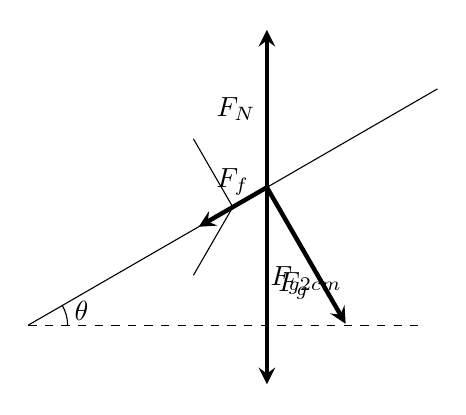
\begin{tikzpicture}

% Define some lengths for the forces
\def\gravity{2.5cm}
\def\normal{2cm}
\def\friction{1cm}
\def\parallel{2cm}

% Draw the inclined plane
\draw (0,0) -- (30:6cm);
\draw[dashed] (0,0) -- (5,0);

% Draw the box
\draw (30:3cm) -- ++(120:1cm) -- ++(-60:1cm) -- ++(-120:1cm) -- cycle;

% Draw and label the forces
\begin{scope}[ultra thick,->,>=stealth]
    \draw (30:3.5cm) -- ++(90:\normal) node[midway,left]{$F_N$};
    \draw (30:3.5cm) -- ++(-90:\gravity) node[midway,right]{$F_g$};
    \draw (30:3.5cm) -- ++(210:\friction) node[midway,above]{$F_f$};
    \draw (30:3.5cm) -- ++(-60:\parallel) node[midway,below]{$F_{g\parallel}$};
\end{scope}

% Label the angle of inclination
\draw (0.5,0) arc (0:30:0.5cm);
\node at (15:0.7cm) {$\theta$};

\end{tikzpicture}
\end{document}